\documentclass[12pts]{article}

% pseudo Times New Roman
\usepackage{mathptmx}% http://ctan.org/pkg/mathptmx
% margins 1 in
\usepackage[a4paper, margin=1in]{geometry}
%line space
\renewcommand{\baselinestretch}{1.5}
% APA citations
\usepackage{apacite}
% math symbols
\usepackage{amssymb}
% tables created in rmd
\usepackage{longtable}
%math 
\usepackage{amsmath}
%images 
\usepackage{graphicx}
\usepackage{subcaption}

%opening
\title{QUANTAL RESPONSE EQUILIBRIUM IN A CITIZEN-CANDIDATE EXPERIMENT}
\author{Alexander Elbittar \and Andrei Gomberg \and Dario Trujano Ochoa}
\date{2018}

\begin{document}

\maketitle

\begin{abstract}

In this study, a Citizen-Candidate model of political competition was implemented in an experiment and the Quantal Response Equilibrium (QRE) was adjusted to data. 
This model of elections is based in the Hotelling-Dows model of spatial competition. 
However, candidates do not choose location, which in this case was their own ideal point, but to campaign or not. QRE is a generalization of the Nash equilibrium (NE) and player's responses are random. Six experimental conditions combine two entry cost levels, 
two voting systems (plurality rule and run-off), and three set of ideal points. 
The Nash Equilibrium (NE) is a good ex ante prediction in all games. 
Though, it cannot predict the large rate of participation nor the changes related to costs and ideal positions.  
In summary,  experimental  data  was explained  by QRE which assumes  a  stochastic  non-perfect  maximizing  decision rule when adjusted by game. However, in one game, the parameter that measures maximizing behavior was high compared with other games.


\end{abstract}

\section{Introduction}

% why is it worth to know
In any democracy, politicians have to decide if they run for office before elections. We suppose they consider payoffs and chances to win which, ultimately, depend on electoral preferences and who their adversaries are going to be. 
However, few people would affirm that politicians are completely predictable, i.e., choosing always the more profitable option, as assumed in Nash equilibrium (NE) calculations.
If we want to understand and predict who will campaign, we need a model of how the political process works and a theory that convey more realistic assumptions of candidates. 
In order to do this, the Citizen-Candidate model proposed by \citeA{Osborne1996} was evaluated experimentally and the results analyzed with the QRE \cite{McKelvey1995,Goeree2016} which relax the perfect maximizing assumption.

This work is located at the intersection of two perspectives:
first, Behavioral Game Theory \cite{Camerer2003a, Gachter2004}, from where QRE was proposed; 
and second, Political Economy \cite{Besley2007}, where the citizen-candidate model is an important instance.
%The implementation of QRE to refine the predictions of the citizen candidate model is the theoretical innovation achieved in this thesis.
%Finally, an important trait to note is the experimental which is the methodological approach used in this thesis. %experimental literature
%I conclude that, considering stochastic and non-perfect maximizing decision rule, it is possible to better describe candidates' decisions in the experiment.

%relation with others empirical studies in political economics
In political economics, it is more common to study voters' behavior \cite{Besley2007}, and candidates' behavior is frequently studied to test median voter theorem under different assumptions \cite{Palfrey2009}. 
Hotelling-Downs model is one the main formal tools to model candidates behavior. In the classical setting, two political options are located on an interval that represents voters' preferences. Each voter chooses the closest candidate to them. Thus, candidates do better as closer to each other and move towards the median if standing in the same position seeking to lure more votes.
In contrast with this model, the Citizen-Candidate model proposed by \citeA{Osborne1996} considers candidate's ideal policy and, once in office, they choose their preferred policy. This model has been empirically implemented by \citeA{Cadigan2005, Elbittar2009}. 
They compared the results with NE and concluded that observed behavior approaches to it, although there are facts that can not be understood under this framework. %Considering more realistic assumptions about behavior lead to more precise description and understanding of equilibrium outcomes seen in other experiments \cite{Goeree2003}, and these results can be applied to real settings with more reliance.

% methodological justification
Elections are clearly modeled with game theory; rules are explicit for voters and candidates.
The objective of political competition models is to determine who will campaign, predict the winner, and the public policies implemented, i.e., NE of the election game.
The experimental approach is advisable to evaluate the effect of relevant variables, and consider the structure of the political process.
Observational data is frequently noisy and/or do not show variance in the key parameters of the model. Particularly, the voting rules are not commonly changed. For this reason, experiments are now part of the basic tools in political economics investigation \cite{Palfrey2009}.

In the experiment, costs of entry, different electoral systems and set of ideal points were modified to evaluate the predictions of the model.
The experimental implementation was exactly the same as that used by \citeA{Elbittar2009} who also analyzed two of the six games presented here without adjusting the QRE.

The Citizen-Candidate model assumes voters' preferences across an unidimensional line in $\mathbb{R}$, as the Hotelling-Downs model.
The decision of campaign depends on the campaign cost, winning benefits, the voting system and the specific set of possible candidates. 
The general model allows any citizen to participate in the competition. 
However, in the experiment, only a finite subset of citizens have this possibility. \footnote{This can be due to barriers, v.g., highly enough costs for the others citizens.} 
The prediction of this model is behavior in line with NE. However, there is great variability within the responses of each individual and a tendency to over-participate was reported by \citeA{Elbittar2009}. 
In the same article, Quantal Response Equilibrium was proposed as a possible tool to explain this phenomenon.

% citizen-candidate model
%Elections entail a number of citizens choosing who will make the decisions among a diversity of candidates and campaign promises, 
%and there are different determinants of participation: cost of campaign, benefits of being elected, characteristics of the candidates, and different electoral systems.

% QRE description
Frequently, we observe others behaving as if randomly and make decisions even against their own benefit. 
We should concern about this during interactions, when others' decisions impact our own welfare. 
In consequence, we must take into account the possibility of others' mistakes and our own behavior. 
However, decisions are not as erratic as they seem: 
we expect others -and ourselves- to commit less mistakes when payoffs are bigger. 
%Also, it is expected people to be more prone to choose better options, even when there is always the possibility that they choose the worst.
These characteristics are captured by QRE in what is called a regular response function (or stochastic best response) which states a mixed strategy profile: 
probabilities of every possible action to be chosen given their expected payoffs. 
A regular response function generalizes best response correspondence in classical game theory, and the concept of equilibrium is completely analogous: 
a point where beliefs and strategies coincide for every player.

% conceptual relevance
The QRE theory considers that agents have certain level of rationality: they are not perfect maximizers, but they are strategic, i.e., they think about others' actions and randomness. 
In this theory, NE is a especial case with perfectly maximizers agents. % citation 
Evaluation of QRE in the context of elections presents an opportunity to check for robustness of the theory and its assumptions, 
whereas providing a more reliable prediction of elections. 



%Elections is the more characteristic trait of any democracy. Many person in the world has been in contact with this practice\footnote{49.3\% of the world population live in a full or flawed democracy according to the Democracy Index}. 
%Furthermore, it is common that in public and private organization some type of democratic process took place time to time. 
%Considering the impact that this kind of process have over the social welfare, a better understanding of democracies seems important and interesting.

%Therefore, the other important objective of this thesis is to explore whether the QRE model can explain the behavior observed in the experiment. Although, it is important to mention that this model is based on the comparison between expected utilities of the options which requires an utility function that, if not linear, affects the predictions. \citeA{Goeree2003}, and \citeA{TrujanoOchoa2013a} found that considering a concave utility function improves the fit of the model.

%main results consistent with conclusions

% Sonia's comments

%Resaltar la importancia del problema de investigación
%Buscar definición de democracia de otra fuente
%RElavancia de estudiar por qué el ciudadano decide entrar a competir para UN PUESTO DE ELECCIÓN POPULAR
%Dejar clara la pregunta de investigación
%relavancia y problemas del modelo de citizen-candidate
%relevancia del fenomeno observado (costos de entrada, quiza perdida de bienestar?)
%





\section{Model}

%The Citizen-Candidate (Osborne and Slivinski 1996) model of political competition is described in detail.

The Citizen-Candidate model assumes that preferences can be represented
in the real line following the Hotelling-Downs's location model. It is
common to normalize preferences in the \([0,1]\) interval but, according with the
empirical setup of the model, the interval \(A=[0,100]\) was considered.
The empirical model was implemented in this fashion: the discrete subset
\(Q={q_1, ..., q_n}, q_i \in A\) represents ideal policies, and each
citizen can be referred to by their ideal which is indicated
exogenously.

Possible candidates consider the cost of participation \((c)\), the
possible benefits of being elected or ego rent \((b)\), and their
preferences over the possible final policies implemented. In order to
model these considerations, equation \ref{eq:Utility} represent the preferences of citizens:

\begin{equation}
u_i(x,q_i)=
\begin{cases}
-D, & \text{if } s_i=0, \forall i \in Q \\
-\alpha||x-q_i|| - cs_i + bw_i(s), & \text{otherwise} 
\end{cases}\label{eq:Utility}
\end{equation}

The parameter \(\alpha\) indicates the importance of the final policy
chosen. Citizen lose utility proportionally to the distance from their ideal point (\(q_i\)).
Thus, citizens prefer policies closer to their locations. The variables
\(s_i \in \{0,1\}\) and \(w_i \in \{0,1\}\) stand for the entry decision
(\(entry=1\), $not entry = 0$), and the final result (\(win=1\), $lose=0$), respectively. Notice
that winning depends on the voting system and the profile of decision
made by citizens (\(s \in \Pi s_i\)), which defines the candidates set.

\subsection{Electoral Systems}\label{electoral-systems}

In this model, sincere voters are considered. Thus there is not the possibility to create coalitions, and each candidate get the voters closest to them.  

\begin{itemize}
	\item \textbf{Plurality Rule}:
	In this System, the candidate who get more votes, calculated as in the Hotelling-Downs's location model, is elected. 
	In the case of a tie the winner is chosen randomly as stated before.
	\item \textbf{Runoff}:
	This system take the two candidates with highest votes from a first round, and then a second round of voting is held only with this two options. In the case that one candidate got more that a half of the votes in the first round, she wins without a second round. Winner is chosen randomly if there is a tie in the second round.
\end{itemize}

\subsection{Stages}\label{stages}

Following (Besley and Coate 1997) the three stages of the elections (entry, voting and policy choice) are
presented in inverse order. This clarifies the subsequent Nash Equilibria
calculus as a consequence of backward induction reasoning.

\subsubsection{Policy Choice}\label{policy-choice}

Once having won and holding the office, winner candidate (\(q_i^*\)) can
implement any policy. It is clear that any
winner will choose their ideal policy (\(x=q_i^*\)) maximizing equation
\ref{eq:Utility}. Therefore, we can define
\(x: q \in Q \rightarrow [0,100]\).
It will be clear that \(x\) is a random variable while \(w\) is drawn
from a set of winner candidates.

An important assumption is perfect information: all players and voters know the
preferences of others which means that candidates cannot lie about
the policy they is going to implement once in office. 
These assumptions, contrast with the classical
Hotelling-Downs model where candidates freely move along the preferences and are enforced to keep their campaign promises.

\subsubsection{Voting}\label{voting}

Given the subset of citizens who have decided to participate in the
election (\(C \subseteq Q\)), there is a voting system that designates
the winners set (\(W: C \rightarrow C\)). Plurality Rule (PR) or Run-off
(RO) determine function \(W\). In both systems, when two or more
candidates get the same number of votes, and more than others, they
belong to \(W\) from were \(q*\) is randomly sampled. In both cases, it
is assumed that the distribution of voters over \(A\) is uniform.
Citizens vote sincerely and choose the closer candidate to their own
location. Furthermore, given that there is a continuum of voters, each
citizen represent a single point in \(A\), then their own vote choice is
negligible\footnote{Remember that there is a continuum of voters from
	which only a discrete subset of them could be candidates referred to
	as citizens.}. The assumption of sincere vote does not allow for
coordination between voters (check Federssen et al 1990).

\subsubsection{Entry}\label{entry}

Each citizen decides simultaneously whether to campaign. They do so
thinking strategically: considering what other citizens would do
evaluating expected payoffs and also thinking strategically. Therefore,
the resulting set \(C\) is a NE. %Now I continue with the construction of expected utility function.

In the case where no citizen presents a candidacy, everyone receives a
payoff of \(-D\) which is high enough to deter this case from the
equilibrium set. Also, note that the cardinality of \(W(C)\) could be more than 1
(\(\#((W(C)) \ge 1\)). In such a case, the winner is chosen with equal
probability due to sincere voting. Then, the citizen \(i\)'s probability
of being elected is defined: \(P_i(C)=1/\#((W(C))\) if \(q_i \in W(C)\)
and \(0\) otherwise. Therefore, the winner is a random variable.

In consequence, given the vector of parameters
\(\theta= (\alpha, c, b, D)\), the expected utility for each citizen can
be defined.

\begin{equation}
U_i( C;\theta )=\Sigma P_j(C)(u_i(x=q_j,q_i;\theta))
\end{equation}

\label{eq:EU}

Because the candidates set is defined from the preceding entry decision
(\(C=C(S)\)), it is convenient to write the expected value as a function
of the profiles:

\[
U_i(s), s \in \Pi_{i \in N} S_i
\]

Now, lets define the best response correspondence as: 
$$BR_i(s)=argmax_{S_i}\{U_i(s)\}$$

From this equation, the existence of a NE can be shown in a standard way
using the fixed point theorem. Considering the points $(s*)$ where $(BR_1(s*),..., BR_n(s*)) = s*$

\section{Experimental Design}\label{experimental-settings-games}

The six experimental treatments had three candidates with different ideal points from the interval $[0, 100]$ which represents the sincere voters.
The six different games were built from 2 entry costs, 2 voting rules and 3 ideal points sets.
Table \ref{tab:parameters} summarizes each game parameters. 
The last three columns show the ideal points labeled \emph{Left}, \emph{Center} and \emph{Right} according with the relative position held by each candidate. The last four game have the same ideal position and were built from crossing costs $5$ and $20$ with the two voting rules. 

\begin{table}[!htbp] \centering 
	\caption{Parameters in the six treatments} 
	\label{tab:parameters} 
	\begin{tabular}{@{\extracolsep{5pt}} ccccccccc} 
		\\[-1.8ex]\hline 
		\hline \\[-1.8ex] 
		Games & VotingRule & alpha & costs & benefit & D & Left & Center & Right \\ 
		\hline \\[-1.8ex] 
		ex70 & Plurality Rule & $0.100$ & $5$ & $25$ & $40$ & $30$ & $50$ & $70$ \\ 
		ex80 & Plurality Rule & $0.100$ & $5$ & $25$ & $40$ & $30$ & $50$ & $80$ \\ 
		PR\_LC & Plurality Rule & $0.100$ & $5$ & $25$ & $40$ & $20$ & $30$ & $80$ \\ 
		PR\_HC & Plurality Rule & $0.100$ & $20$ & $25$ & $40$ & $20$ & $30$ & $80$ \\ 
		RO\_LC & Run-Off & $0.100$ & $5$ & $25$ & $40$ & $20$ & $30$ & $80$ \\ 
		RO\_HC & Run-Off & $0.100$ & $20$ & $25$ & $40$ & $20$ & $30$ & $80$ \\ 
		\hline \\[-1.8ex] 
	\end{tabular} 
\end{table} 

\subsection{Participants}

For each game there were three sessions with different participants who were students of various undergraduate programs at ITAM in Mexico City. They played three practice trials at the beginning of each session and at most during 30 effective trials.
Participants were randomly matched and assigned an ideal point each trial. 
Less trials happened if participants lost all the money given or because there were a non-multiple of three; then, one or two participants waited until the next trial-match. 
Each one initiated with $\$140$, this amount changed through the session according with the payoffs. Participants were allowed to continue until they finished a trial with negative balance. 

\subsection{Nash Equilibria}

There are only two possible equilibria:

\begin{itemize}
	\item One-Candidate Equilibrium:
		$s_i=1, s_{-i}=0$
	\item Two-Candidate Equilibrium:
		$s_i=s_j=1, i \neq j, s_{k}=0, \forall k\neq i,j$
\end{itemize}

The Nash equilibria in pure strategies are stated in table \ref{tab:equilibria}. The only games with two-candidate equilibrium are \emph{ex70} and \emph{PR\_LC}, which are those with low cost, extreme ideal points symmetric around median and voting  plurality rule. The closest equilibrium to empirical proportion of entering are marked with an asterisk. 

\begin{table}[!htbp] \centering 
	\caption{Possible equilibria with the ideal points of entering candidates}
	\label{tab:equilibria} 
	\begin{tabular}{@{\extracolsep{5pt}} ccc} 
		\\[-1.8ex]\hline 
		\hline \\[-1.8ex] 
		Games & OneCandidate & TwoCandidate \\ 
		\hline \\[-1.8ex] 
		ex70 & $50$ & \textbf{30*, 70*} \\ 
		ex80 & \textbf{50*} &  \\ 
		PR\_LC & \textbf{30*} & $20$, $80$ \\ 
		PR\_HC & \textbf{30*} &  \\ 
		RO\_LC & \textbf{30*} &  \\ 
		RO\_HC & \textbf{30*} &  \\ 
		\hline \\[-1.8ex] 
	\end{tabular} 
\end{table} 

\subsection{QRE}\label{qre}

The Quantal Response Equilibrium (QRE) proposed by (Richard D McKelvey
and Palfrey 1995) is constructed on the base of a stochastic best
response function. The most used implementation is the logistic function
over the difference between the expected payoff of the options:

\begin{equation}\label{fn:SBR}
\sigma_{ij}= \displaystyle\frac{e^{(\pi_{j})\lambda}}{e^{(\pi_{j})\lambda}+e^{(\pi_{i\ne j})\lambda} } 
=\displaystyle\frac{1}{1+e^{(\pi_{i\ne j}-\pi_{j})\lambda }}        
\end{equation}

The degree of stochasticity in the electionis determined by \(\lambda\). When
\(\lambda \rightarrow 0\) the election is a fair coin tossing for each
option independent of the expected payoffs (minimum level of
rationality), and when \(\lambda \rightarrow \infty\) the election is
deterministic with the more profitable action being chosen with
certainty (complete rationality). The expected payoff of action \(j\) is
represented by \(\pi_j\). Notice that $\pi_j: \sigma_{-i} \rightarrow \mathbb{R}$, where $\sigma_{-i}$ stands for others' distribution of probability.

An easy way to visualize the effect of \(\lambda\) over decisions is to
remember the logistic regression: the dependent variable is the
probability to choose option \(j\), and the independent variable is the
difference between expected payoffs of the two options. Intercept is
fixed in zero -which imply equal probability when options' expected
payoffs are the same-, and slope is precisely \(\lambda\), what
determines how step is the logistic function. For this reason,
\(\lambda\) is also interpreted as the level of rationality: as it
increases, decision will be better in terms of expected payoffs and less
uncertain.


With equation \ref{fn:SBR} a stochastic best response is defined:

\begin{equation}
\sigma^*_{ij}(\lambda, \beta, \pi_{j}(\sigma_{-i}))
\end{equation}\label{eq:SBR} 

, which is the player \(i\)'s probability of choose the
actions \(j\) (i.e.~Entry or Not Entry in the Citizen-Candidate model).
Vector \(\beta\) commonly refers to economic parameters that can measure
risk aversion or altruism. In the present analysis, I do not consider
these possibilities, but because \(\beta\) refers to changes in the
original payoff matrix, I will use \(\beta\) to refer to different
games.

With equation \ref{eq:SBR}, a distribution over actions for each player
is defined: \[\sigma^*_{i}(\lambda, \beta, \sigma_{-i})\]

This stochastic best response have the proprieties of a regular quantal
response function stated by (Goeree, Holt, and Palfrey 2016):

\begin{itemize}
	\item Interiority: $\sigma_{ij} >0$
	\item Continuity: $\sigma_{ij}$ is continuous and differentiable. 
	\item Responsiveness:  $\partial \sigma_{ij} / \partial \pi_{ij} >0 $
	\item Monotonicity: $\pi_{ij}> \pi_{ik} \Rightarrow \sigma_{ij}>\sigma_{ik}$
\end{itemize}

Notice that stochastic best response is a function of others' mixed
strategies (\(\sigma_{-i}\)). This is the case because, as seen in
equation \ref{fn:SBR}, probability depends on \(\pi_{j}\) which is a
function of others' strategies: \(\pi_{j}(\sigma_{-i})\). In the case of
the Citizen-Candidate model, \(\pi_j\) is the expected payoff of
equation \ref{eq:EU}.

Define then the function:

\begin{equation}\label{eq:sigma}
\sigma = (\sigma^*_{1}, ..., \sigma^*_{N})
\end{equation}

Then, quantal response equilibrium (\(\sigma^*\)) is a fixed point of
equation \ref{eq:sigma}, that now is a function only of \(\lambda\) and
\(\beta\). Due to the proprieties of the stochastic best response, and
using the fixed point theorem, the equilibrium existence is assured.
The QRE can be seen as the solution of a non-linear system of equations which is solved numerically. 

Note that a different equilibrium is predicted depending of the value of
\(\lambda\) and that players tend towards pure strategies as \(\lambda\)
goes larger. This equilibrium is called logit equilibrium (Goeree, Holt,
and Palfrey 2016). The software Gambit (Richard D. McKelvey, McLennan,
and Turocy 2014) allows to see those equilibria as a function of the
rationality parameter \(\lambda\). I realized the calculus in \emph{R}
(R Core Team 2017) with the package \emph{nleqslv} (Hasselman 2017), and
compare the result with gambit's; they are the same.



\section{Results}


\begin{table}[!htbp] \centering 
  \caption{Characteritics by Sessions} 
  \label{} 
\begin{tabular}{@{\extracolsep{5pt}} cccc} 
\\[-1.8ex]\hline 
\hline \\[-1.8ex] 
Treatmet & Sesion & No.Participants & Bankrupcy \\ 
\hline \\[-1.8ex] 
PL & $1$ & $19$ & $0$ \\ 
PL & $2$ & $18$ & $0$ \\ 
PL & $3$ & $20$ & $0$ \\ 
PH & $1$ & $15$ & $9$ \\ 
PH & $2$ & $20$ & $13$ \\ 
PH & $3$ & $23$ & $16$ \\ 
RL & $1$ & $26$ & $0$ \\ 
RL & $2$ & $16$ & $0$ \\ 
RL & $3$ & $27$ & $2$ \\ 
RH & $1$ & $15$ & $4$ \\ 
RH & $2$ & $15$ & $5$ \\ 
RH & $3$ & $15$ & $6$ \\ 
PLCS & $1$ & $21$ & $1$ \\ 
PLCS & $2$ & $15$ & $0$ \\ 
PLCA & $1$ & $21$ & $0$ \\ 
PLCA & $2$ & $15$ & $0$ \\ 
\hline \\[-1.8ex] 
\end{tabular} 
\end{table} 


In the table \ref{tab:rawentry}  we can see the total number of entries in each game by each ideal position. The differences among the number of total trials is due to bankruptcy of the participants that could not longer play.


\begin{table}[!htbp] \centering 
  \caption{Total number of entries by position and game} 
  \label{tab:rawentry} 
\begin{tabular}{@{\extracolsep{5pt}} ccccccc} 
\\[-1.8ex]\hline 
\hline \\[-1.8ex] 
Position & PL & PH & RL & RH & PLCS & PLCA \\ 
\hline \\[-1.8ex] 
Left & 254 &  89 & 254 &  82 & 296 & 299 \\ 
\% & (47) & (23.4) & (39.2) & (23.4) & (89.7) & (90.6) \\ 
Center & 468 & 332 & 630 & 337 & 164 & 263 \\ 
\% & (86.7) & (87.4) & (97.2) & (96.3) & (49.7) & (79.7) \\ 
Right & 468 & 218 & 278 &  82 & 297 & 164 \\ 
\% & (86.7) & (57.4) & (42.9) & (23.4) & (90) & (49.7) \\ 
Total & 540 & 380 & 648 & 350 & 330 & 330 \\ 
\hline \\[-1.8ex] 
\end{tabular} 
\end{table} 


\subsection{Distribution of Errors}

Considering how people behave, it is possible to measure the error as the difference between what participants should have done (choose the option with the highest expected payoff) and what they did (proportion of entry). Then, considering the proportion of entry, a negative value means that they enter less than what is optimal, and a positive value means that they over-participate when they should not. In figure \ref{fig:errordist}, it can be seen the distribution of such error by game and position.


\begin{figure}[h]
	
	\begin{subfigure}{0.5\textwidth}
		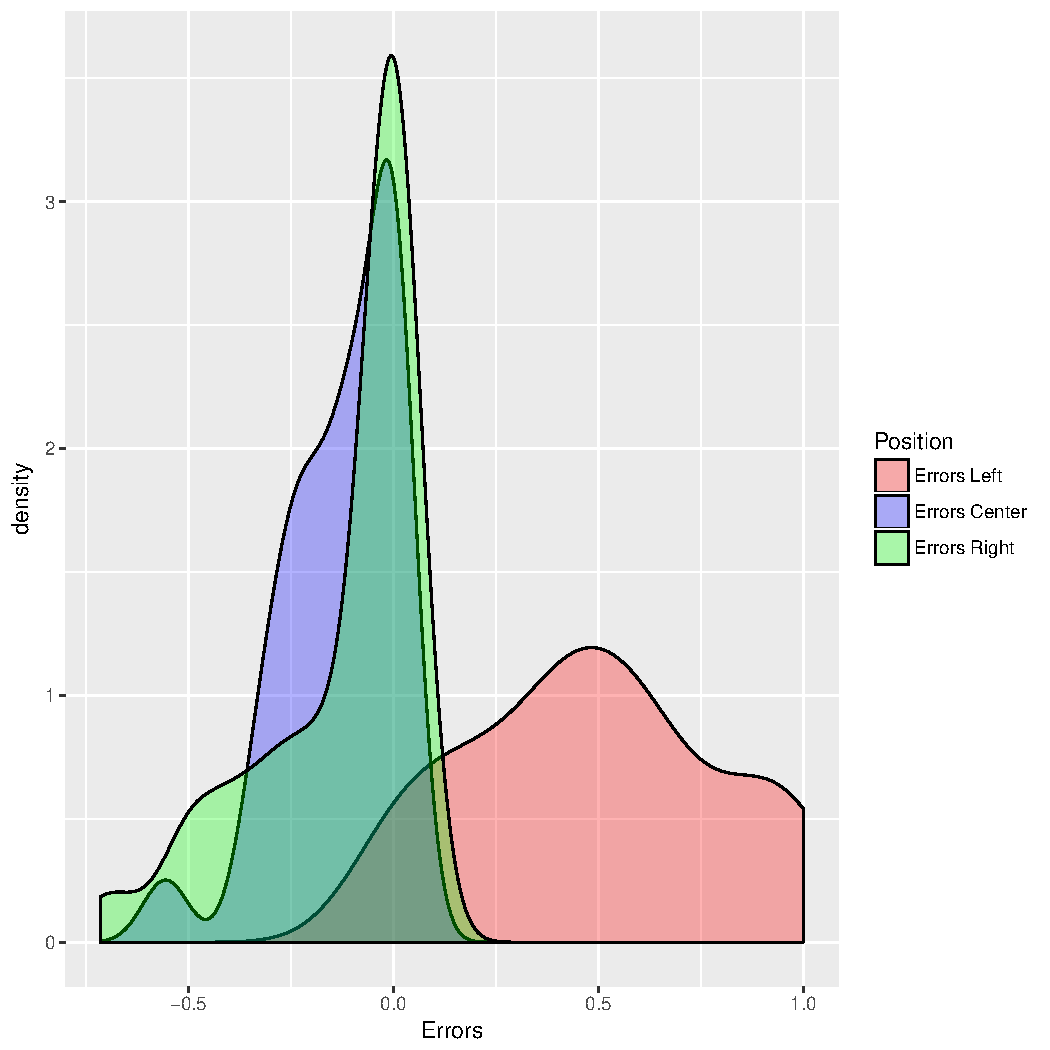
\includegraphics[width=1\linewidth, height=7cm]{../../results/figures/errorDistributionPR_LC} 
		\caption{PR\_LC}
		\label{fig:errdistsubim1}
	\end{subfigure}
	\begin{subfigure}{0.5\textwidth}
		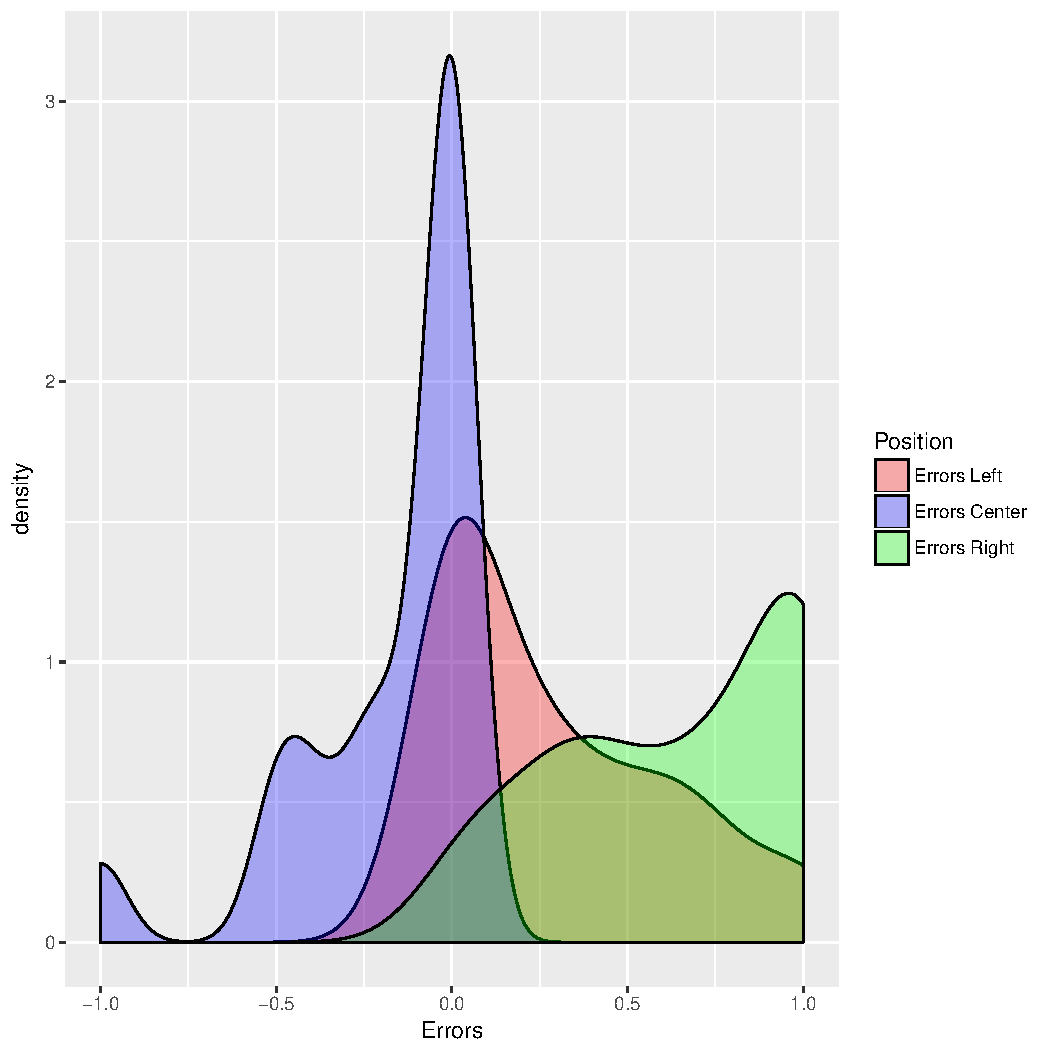
\includegraphics[width=1\linewidth, height=7cm]{../../results/figures/errorDistributionPR_HC}
		\caption{PR\_HC}
		\label{fig:errdistsubim2}
	\end{subfigure}

	\begin{subfigure}{0.5\textwidth}
	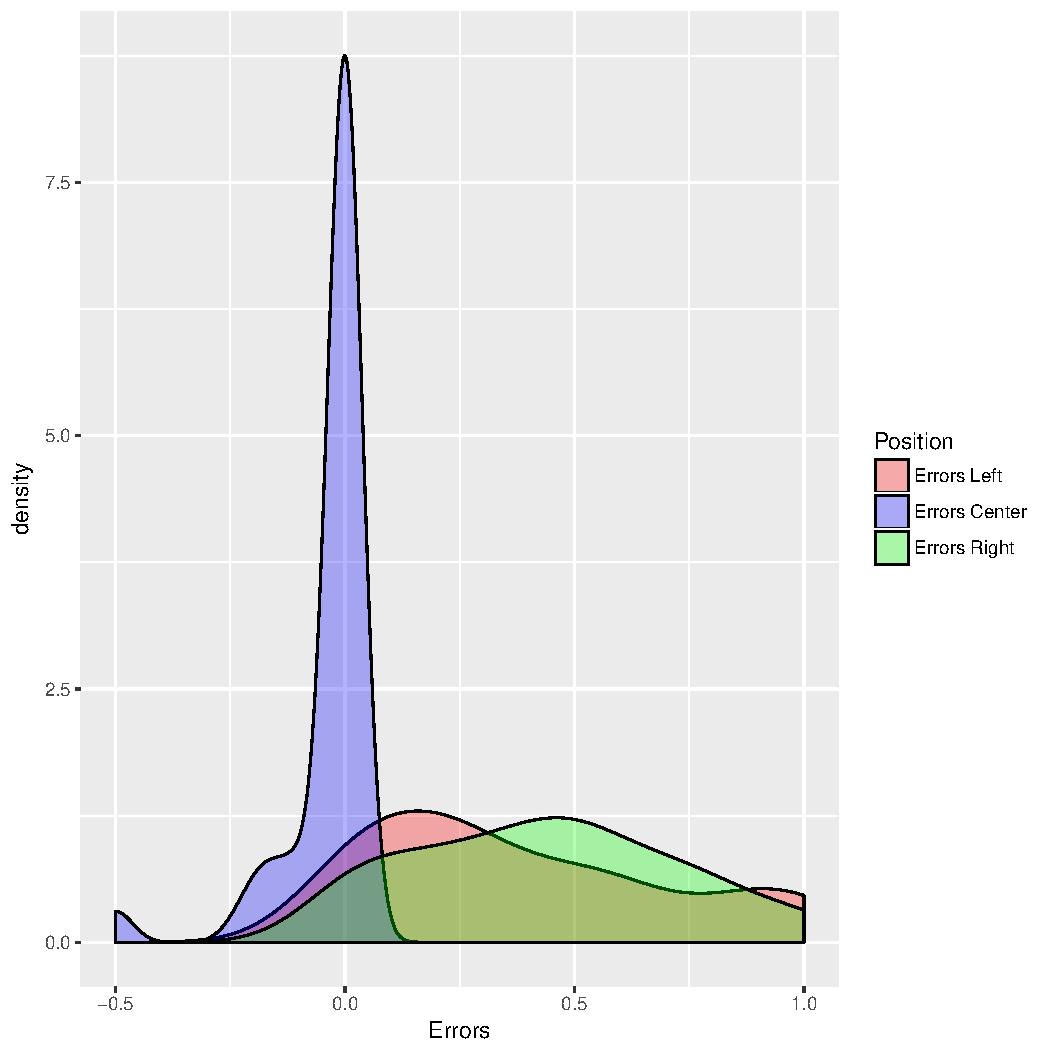
\includegraphics[width=1\linewidth, height=6cm]{../../results/figures/errorDistributionRO_LC} 
	\caption{RO\_LC}
	\label{fig:errdistsubim3}
	\end{subfigure}
	\begin{subfigure}{0.5\textwidth}
	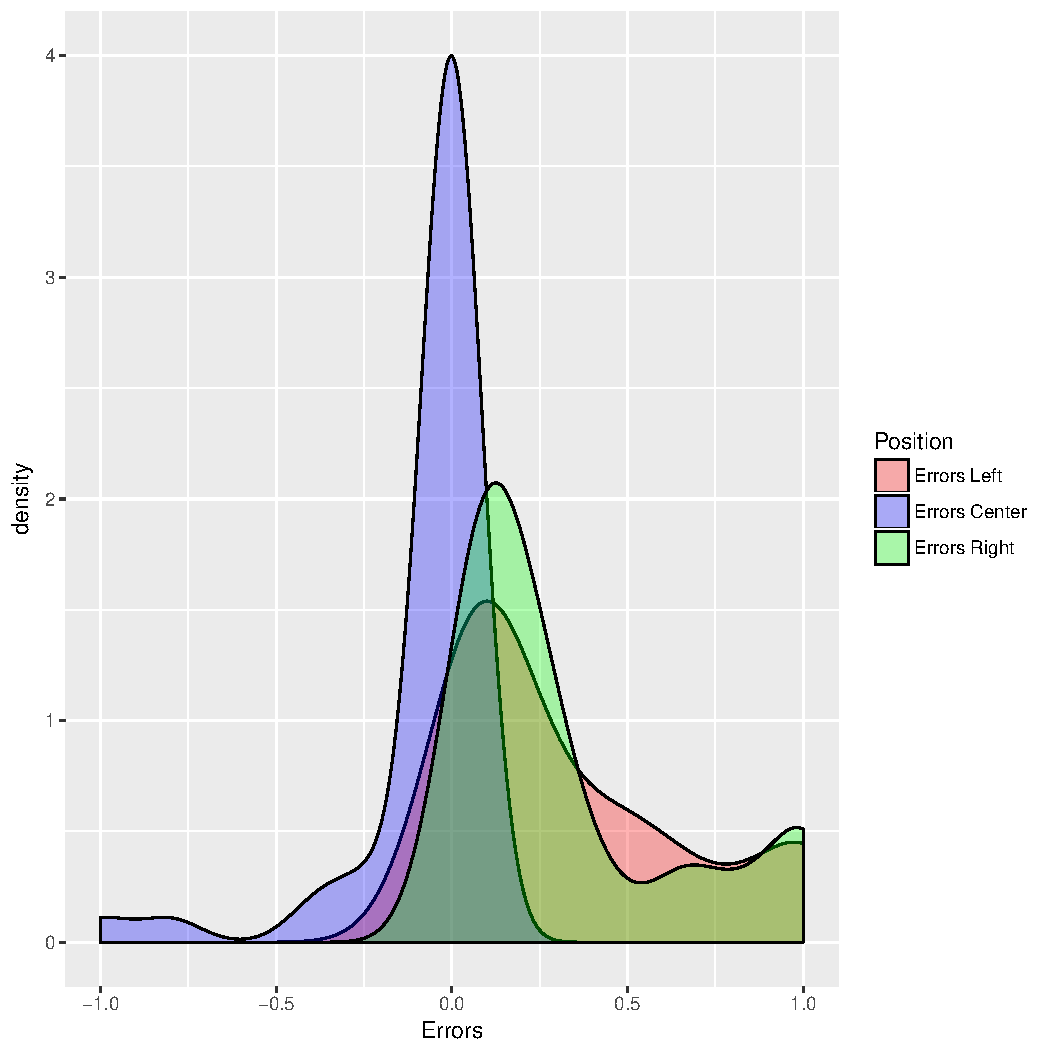
\includegraphics[width=1\linewidth, height=7cm]{../../results/figures/errorDistributionRO_HC}
	\caption{RO\_HC}
	\label{fig:errdistsubim4}
	\end{subfigure}

	\begin{subfigure}{0.5\textwidth}
	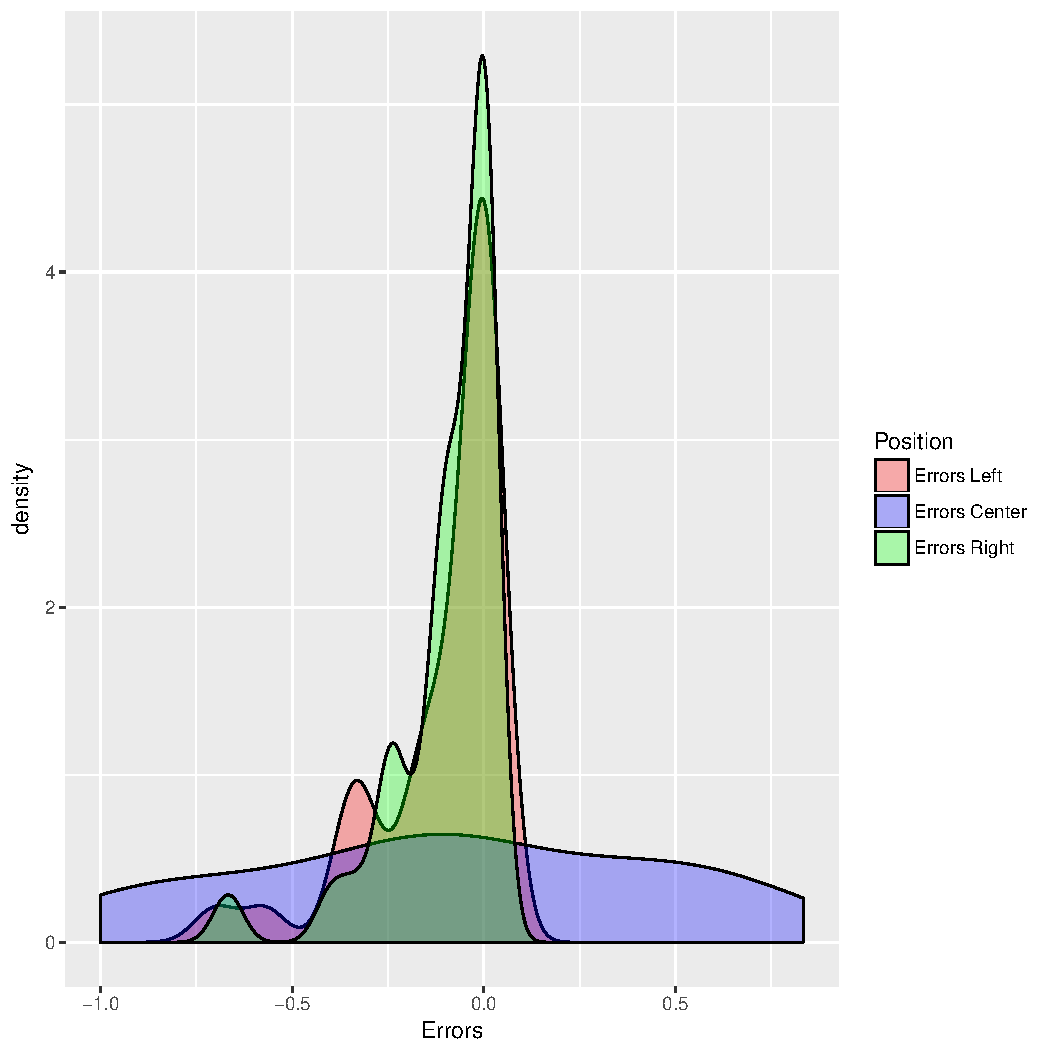
\includegraphics[width=1\linewidth, height=7cm]{../../results/figures/errorDistributionex70} 
	\caption{ex70}
	\label{fig:errdistsubim5}
	\end{subfigure}
	\begin{subfigure}{0.5\textwidth}
	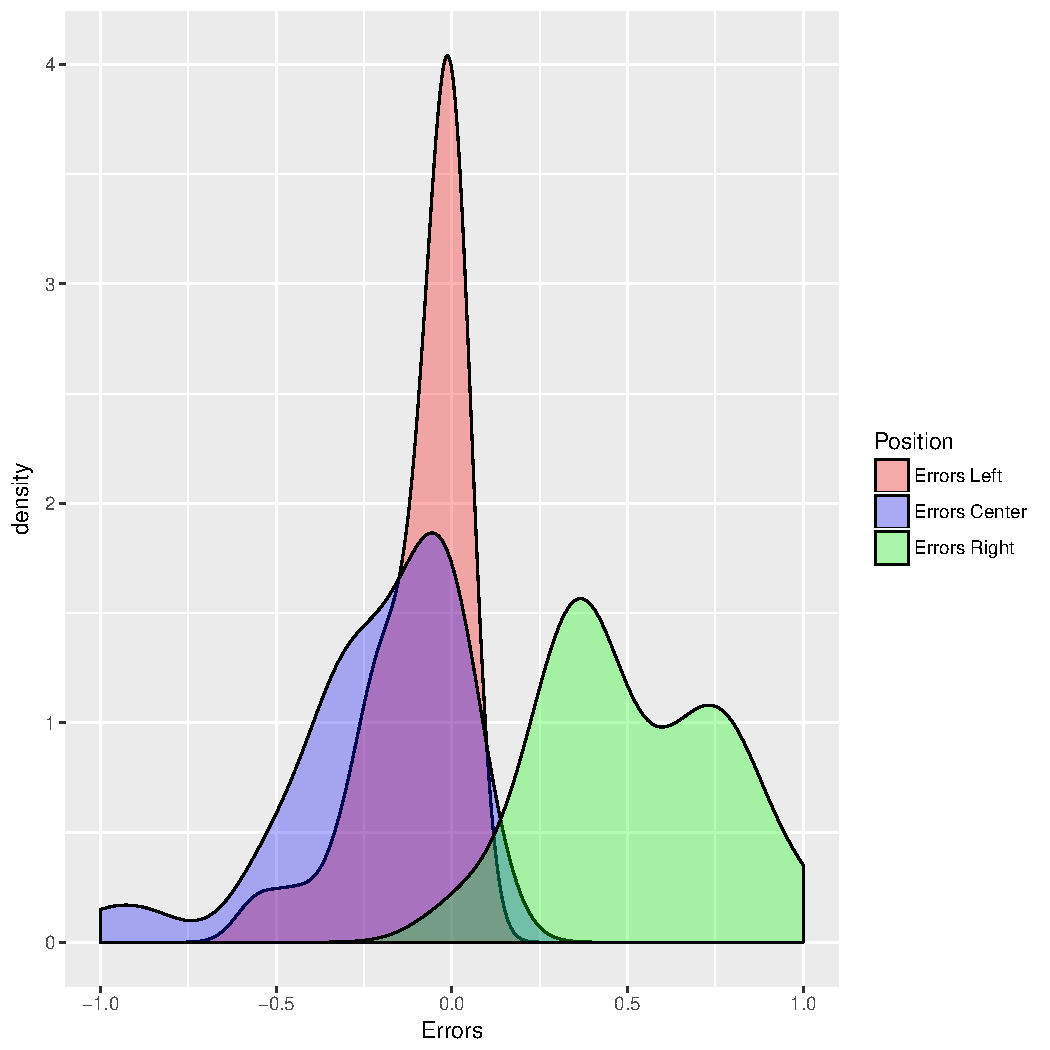
\includegraphics[width=1\linewidth, height=7cm]{../../results/figures/errorDistributionex80}
	\caption{ex80}
	\label{fig:errdistsubim6}
	\end{subfigure}
	
	\caption{Distribution of error by game and position. For each participant, the error was calculated as the difference between the proportion of entry observed and the optimal entry according with the expected payoff calculated based on the entry proportion of all participants in the session.}
	\label{fig:errordist}
\end{figure}


Participants in the central position do not deviate too much from the optimal decision. It is particularly clear in the games whit the same ideal positions $Q=\{20, 30, 80\}$. However, as can be seen in the graph \ref{fig:errdistsubim5}, the behavior in this position is completely random in the game \emph{ex70}, where the extreme positions enter frequently. Furthermore, players in these positions make less mistakes. On the other hand, errors are biased towards over-entering, with some exceptions among participants in the central position. Particularly, in games \emph{PR\_LC} an d\emph{ex80} there is a clear recognition of the over-entering position (figures \ref{fig:errdistsubim1} and \ref{fig:errdistsubim6}). In both cases, that position is the closest to the winning central. This could be due to the fact that, in terms of payoffs, they did not lose too much if the central position wins, but still they continue participating. 



\subsection{Maximul Likelihood Estimation of $\lambda$}

Data analysis at different levels was calculated by maximum likelihood,
following directions from (Goeree, Holt, and Palfrey 2016). The
equilibrium correspondence approach was used: the QRE is calculated for
a given \(\lambda\) and other parameters (\(\beta\)):
\(\sigma*_{ij}(\lambda, \beta)\). In order to find this function, a non
linear equations system with no analytical solution has to be solved.
This was done using the R package \emph{nleqslv} (Hasselman 2017).

Once this function is constructed, it is possible to find the general
logLikelihood objective function, and the then optimize it.

\begin{equation}\label{fn:MLE}
logL(\lambda) = 
\Sigma^n_{i=1} \Sigma^{J_i}_{j=1} f_{i,j} log(\sigma^*_{ij}(\lambda, \beta))
\end{equation}

In the objective function \ref{fn:MLE}: \(n=3\), \(J_i = 2\) and
\(f_{i,j}\) are the times each i-th citizen choose their j-th option. Notice that it was constructed under the assumption of independence of decisions. Also it is assumed that $\lambda$ is the same for all of them.
The Global and by game estimators are in table \ref{tab:mle}.

\begin{table}[!htbp] \centering 
	\caption{} 
	\label{} 
	\begin{tabular}{@{\extracolsep{5pt}} cccccccc} 
		\\[-1.8ex]\hline 
		\hline \\[-1.8ex] 
		X & Global & PR\_LC & PR\_HC & RO\_LC & RO\_HC & ex70 & ex80 \\ 
		\hline \\[-1.8ex] 
		Estimate & $0.078$ & $0.084$ & $0.072$ & $0.098$ & $0.083$ & $0.222$ & $0.075$ \\ 
		sd & $0.001$ & $0.003$ & $0.001$ & $0.004$ & $0.002$ & $0.007$ & $0.004$ \\ 
		\hline \\[-1.8ex] 
	\end{tabular}\label{tab:mle}
\end{table} 

QRE estimation is a punctual number, but the graph of $\sigma (\lambda, \beta)$ can be built for each game. Figure \ref{fig:QRE} displays such function. We can see that when $\lambda=0$ all the players choose entry with $0.5$ probability, and how they approach smoothly towards a some NE. Also, we can see how well the model explain data. Horizontal lines, with their colors corresponding with each player, are the observed proportion in the experiment. Solid vertical line is the global estimate of $\lambda$, and dotted line is the estimation within each game. Where those lines cross is the QRE prediction.

In general, the value of $\lambda$ is similar among games, except for \textit{ex70} game. The estimated is too large compared with the other games, even when it can be seen that prediction is almost perfect. The reasons for this divergence must be investigated more deeply. The worst adjustment is in the \textit{ex80} game where $q_{30}$'s observed proportion of entry is higher than $q_{50}$'s, a fact that QRE cannot explain.

\begin{figure}
	\begin{subfigure}{0.6\textwidth}
		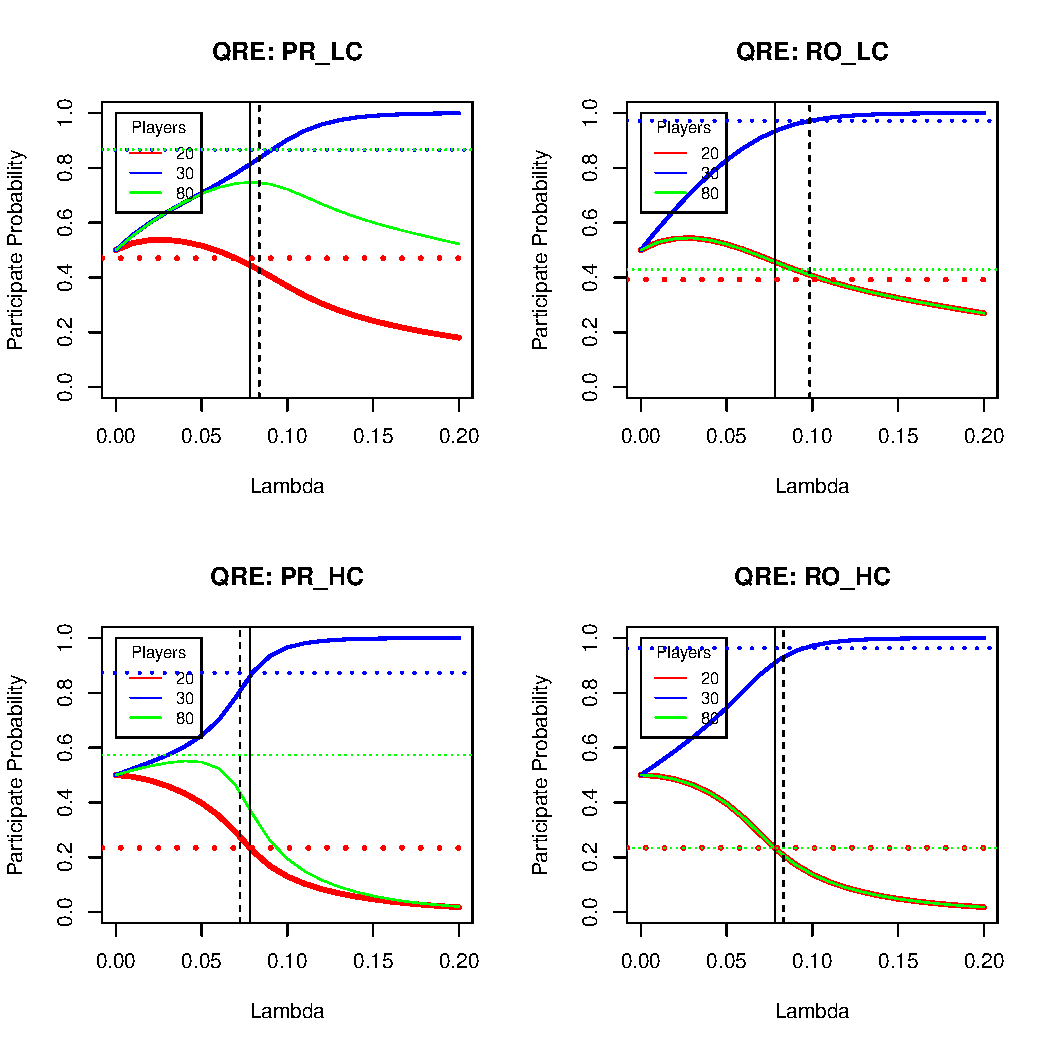
\includegraphics[width=1\linewidth]{../../results/figures/QRE_lambda_MLE}
		\caption{}
		\label{fig:qrelambdamle}
	\end{subfigure}
	\hfill
	\begin{subfigure}{0.7\textwidth}
		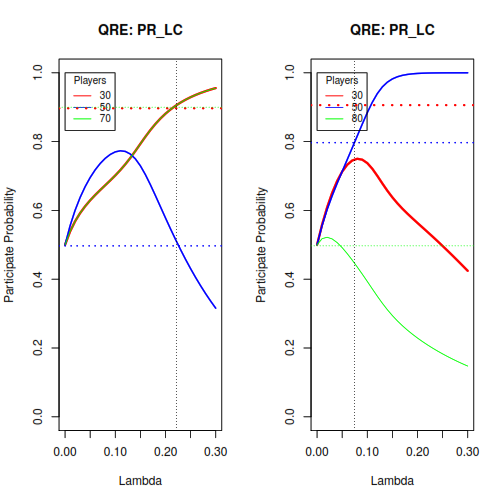
\includegraphics[width=0.6\linewidth]{../../results/figures/1st_treatments_plot}
		\caption{}
		\label{fig:1sttreatmentsplot}
	\end{subfigure}

\caption{QRE expected as a function of $\lambda$}
\label{fig:QRE}
\end{figure}


\subsubsection{Other Equilibria}

Other QRE emerge when $\lambda$ increase if there are other NE because they are especial cases of the QRE when $\lambda\rightarrow\infty$.
When $\lambda$ equals $0$ complete randomness is the only equilibrium, as can be seen in figure \ref{fig:qrelambdamle}. From this point, comes an equilibrium called \emph{logit equilibrium}\cite{Goeree2016}. 
Stochastic best responses seem continuous (even differentiable) functions of the parameter $\lambda$. However, as this parameters increases there will appear other equilibria from anywhere. 

Those equilibria can be seen in figures \ref{fig:ex70eqilibria} and \ref{fig:prlceqilibria}. It is seen as a discrete change in the probability of entry expected for each ideal point. Particularly, in figure \ref{fig:prlceqilibria}, we can see that equilibrium tended towards $q_{30}$ entering alone, and suddenly it is left out the election when $\lambda$ is around $0.15$. On the other hand, in figure \ref{fig:ex70eqilibria}, the contrary pattern is observed when $\lambda$ is around $0.17$.

\begin{figure}[h]
	\begin{subfigure}{0.5\textwidth}
		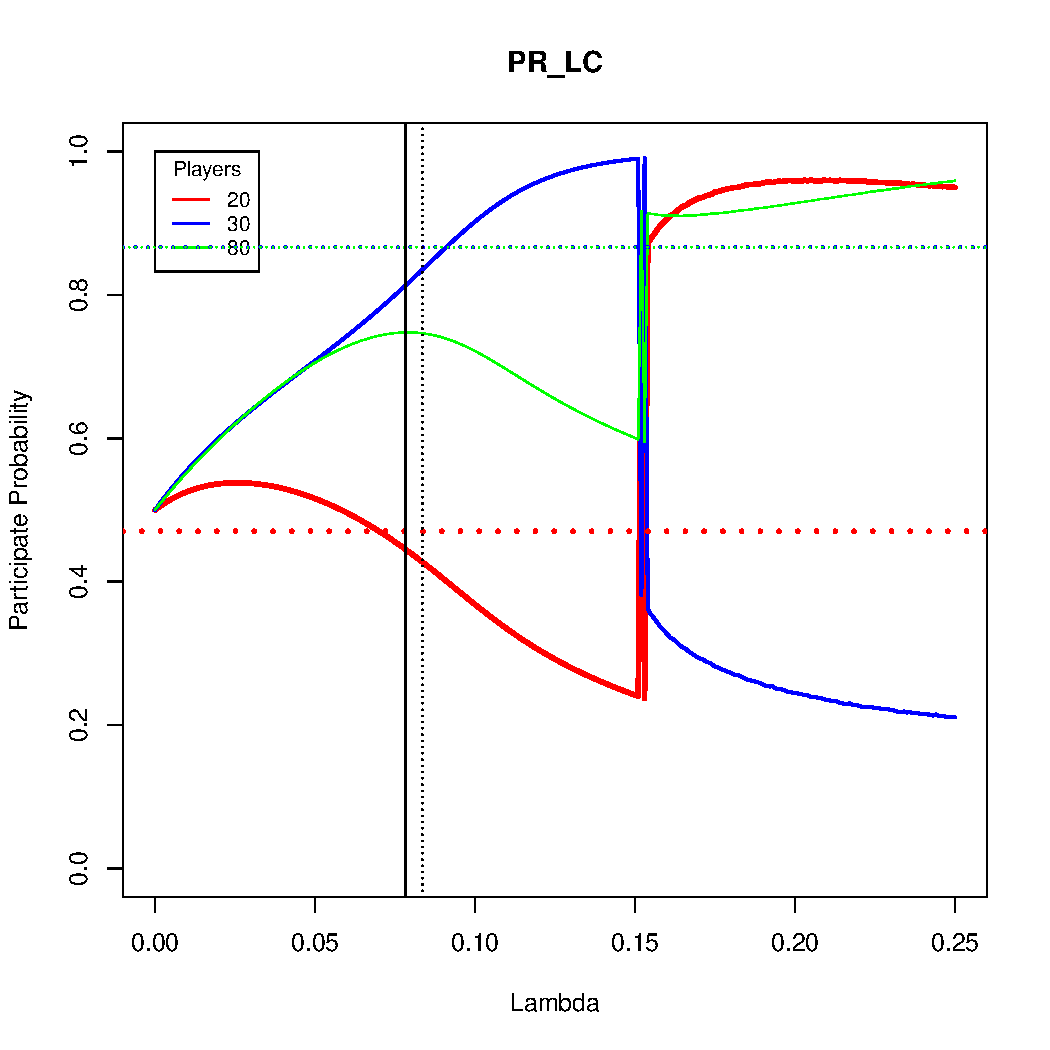
\includegraphics[width=0.7\linewidth]{../../results/figures/PR_LC_eqilibria}
		\caption{}
		\label{fig:prlceqilibria}
	\end{subfigure}
	\hfill
	\begin{subfigure}{0.5\textwidth}
		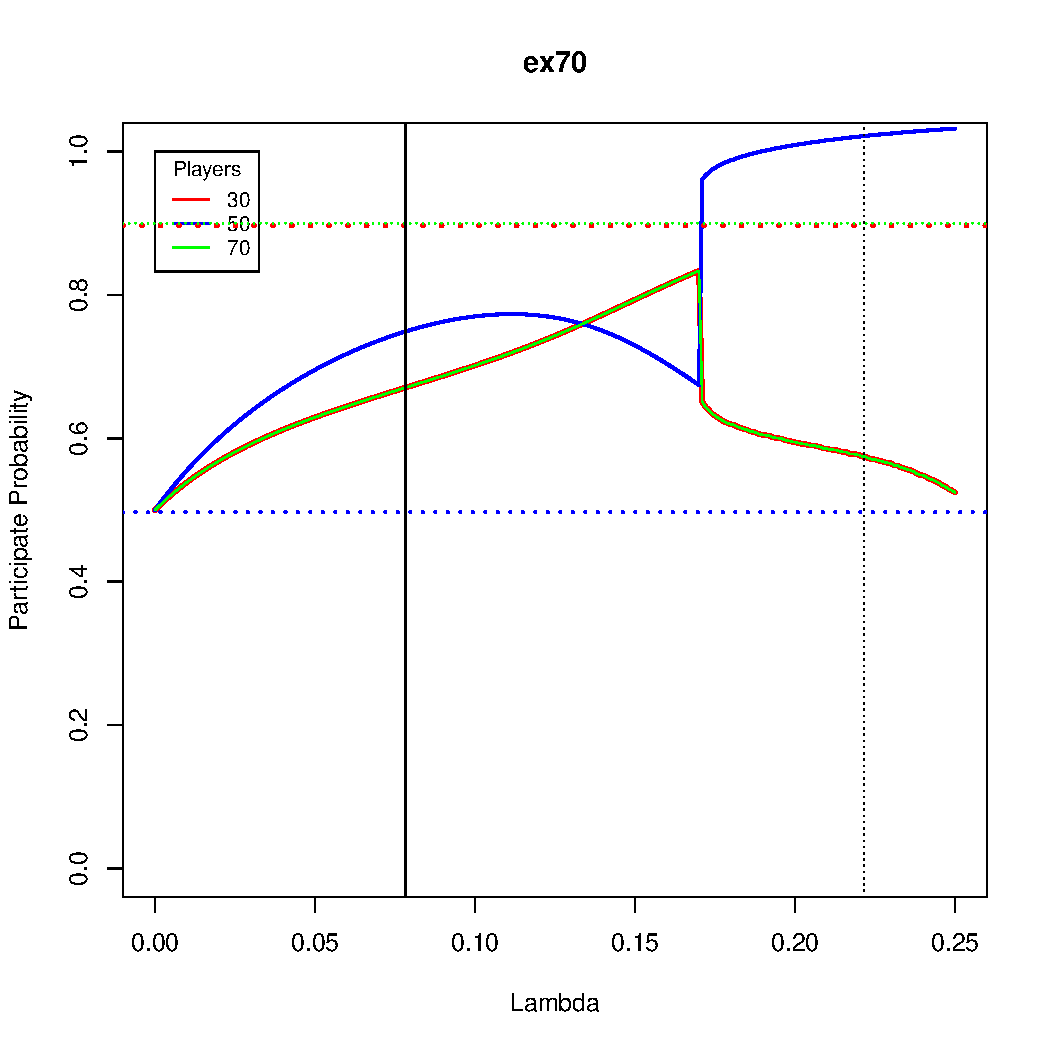
\includegraphics[width=0.7\linewidth]{../../results/figures/ex70_eqilibria}
		\caption{}
		\label{fig:ex70eqilibria}
	\end{subfigure}

\label{fig:otherQRE}
\caption{Other equilibrium that emerge when  $\lambda$ increases.}
\end{figure}


\section{Conclusion}

%Quantal response Equilibrium, which consider stochastic behavior, can describe candidates' decisions in the experiment. 

There is variability in the data that can not be explained by random error alone: there are systematic deviations from the standard prediction of NE that can be explained by QRE theory. This theory considers that participants' decisions depends stochasticity on the expected payoffs they face, which also depend on other's decisions that are also random. If we assume that players consider that others behave in the same way, QRE is the point when strategies and beliefs about strategies are the same.  

Considering that citizen-candidate assumption describe well enough the electoral process, the main prediction of QRE theory is that there are more candidates than expected by standard game theory. % review why there is not less entrance
This is the result of a direct and indirect effect of the stochastic best response. % check for direct and indirect effects of stocastic behavior as derivatives using calculus
First, there is a direct effect of the stochasticity that made the Nash winner ($q_{30}$) less probable to enter and increase the probability of others to enter. 
Second, others candidates increase their expected payoffs to participate because the probability of being defeated decreases relative to NE. % there could be the case of a reversal in a Nash winner strategy?, i.e. QRE for her gives a probability of less than 0.5 % review model of federesen specifically the case when there are many candidates at the median and one diferenciated one. In the present case review for the {20,80} equilibrium 
The magnitude of this indirect effect depends on the citizen's position relative to Nash winner; distant candidates to her are more prone to participate. This implication goes according with data observed.

Notice that the model adjust considerably good in al the experimental treatments when the parameter of stochasticity ($\lambda$) is calculated for those games. This parameter is similar in all games except for one where it is relatively higher. The reasons of this increase of $\lambda$ in this game are unclear. It is possible that it is related with the fact that game \textit{ex70} is the only game with an equilibrium where extreme ideal points enter in a higher proportion.

Finally, it most be noted that NE is not a bad forecasting. Nevertheless, QRE not just offer a more precise description, but also predict other interesting phenomena in data.

\bibliographystyle{apacite} 

\bibliography{library}

\end{document}
